\section{DBSCAN}
DBSCAN jest popularnym algorytmem grupowania gęstościowego. Najważniejsze jego zalety wymienione w \cite{dbscan} to tworzenie grup o dowolnym kształcie oraz możliwość doboru parametrów przy niewielkiej wiedzy o zbiorze danych. Grupy tworzone są na podstawie lokalnej gęstości punktu rozumianej jako liczba punktów w otoczeniu punktu, dzięki czemu tworzone są grupy o intuicyjnych kształtach. Ważną cechą DBSCAN jest też pojęcie punktów szumu, czyli takich, które nie pasują do żadnej grupy. Punkty szumu mogą być cenne, na przykład przy wykrywaniu anomalii.

\subsection{Definicje}

\definition{$ \varepsilon $-otoczenie (ang. $ \varepsilon $-neighbourhood)}\newline
Zakładamy, że grupowany jest zbiór punktów $ D $. Na potrzebę algorytmu definiuje się pojęcie $ \varepsilon $-otoczenia punktu $ p \in D $. Jest to zbiór punktów $ q \in D $ znajdujących się w odległości nie większej niż $ \varepsilon $ od punktu $ p $, dla którego jest wyznaczane $\varepsilon$-otoczenie. Dalej $\varepsilon$-otoczenie punktu $ p $ w zbiorze $ D $ będzie oznaczane $ N_{D,\varepsilon}(p) $.
\begin{equation}\label{eq:eps-neighbourhood}
	N_{D,\varepsilon}(p) = \set{q \in D | d(p, q) \le \varepsilon}
\end{equation}

\definition{punkt rdzeniowy (ang. core point)}\newline
Punkt $ p $, który posiada w swoim $ \varepsilon $-otoczeniu $ N_{D,\varepsilon}(p) $ co najmniej $ \mu $ punktów jest nazywany punktem rdzeniowym ($ core_{D,\varepsilon,\mu}(p) $).
\begin{equation}\label{core-point}
	core_{D,\varepsilon,\mu}(p) \iff |N_{D,\varepsilon}(p)| \ge \mu
\end{equation}

\begin{figure}
	\centering
  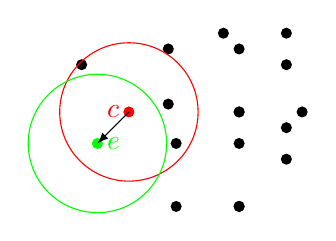
\begin{tikzpicture}
		\fill (-2,1.8) circle(2pt);
		\fill (-.9, 1.3) circle(2pt);
		\fill (-.9,2) circle(2pt);
		\fill (-.8,.8) circle(2pt);
		\fill (-.8,0) circle(2pt);
		\fill (-.2,2.2) circle(2pt);
		\fill (0,0) circle(2pt);
		\fill (0,1.2) circle(2pt);
		\fill (0,1.2) circle(2pt);
		\fill (0,0) circle(2pt);
		\fill (0,.8) circle(2pt);
		\fill (0,2) circle(2pt);
		\fill (.6,1) circle(2pt);
		\fill (.6,.6) circle(2pt);
		\fill (.6,1.8) circle(2pt);
		\fill (.6,2.2) circle(2pt);
		\fill (.8,1.2) circle(2pt);
    
    \fill[red] (-1.4,1.2) circle(2pt) node[anchor=east]{$ c $};
    \draw[red] (-1.4,1.2) circle(25pt);
    
    \fill[green] (-1.8,.8) circle(2pt) node[anchor=west]{$ e $};
    \draw[green] (-1.8,.8) circle(25pt);
    
		\draw[-latex] (-1.4,1.2) -- (-1.8,.8);
		
  \end{tikzpicture}
  \caption{Punkt rdzeniowy $ c $, brzegowy $ e $ oraz relacja bezpośredniej gęstościowej osiągalności $ dirreach_{\varepsilon,\mu}(e, c) $, $ \mu=3$.}\label{fig:core-edge-point}
\end{figure}

\definition{bezpośrednia gęstościowa osiągalność (ang. direct density reachability)}\newline
Dalej, na potrzebę definicji grupy wprowadza się pojęcie bezpośredniej gęstościowej osiągalności. Jest to niesymetryczna relacja, która zachodzi jeśli punkt $ p $ znajduje się w $ \varepsilon $-otoczeniu punktu rdzeniowego $ q $. Punkt $ p $ jest bezpośrednio gęstościowo osiągalny z punktu $ q $, jeśli punkt $ q $ jest punktem rdzeniowym i $ p $ znajduje się w $ \varepsilon $-otoczeniu punktu $ q $ ($ dirreach_{D,\varepsilon,\mu}(p, q) $).
\begin{equation} \label{direct-reachability}
	dirreach_{D,\varepsilon,\mu}(p, q) \iff p \in N_{D,\varepsilon}(q) \land core_{D,\varepsilon,\mu}(q)
\end{equation}
To, że $ p $ jest bezpośrednio gęstościowo osiągalny z $ q $, nie determinuje, \mbox{że $ q $ jest} bezpośrednio gęstościowo osiągalny z $ p $.
\begin{equation} \label{direct-reachability-asymmetry}
	\exists_D\;\neg\forall_{p,q\in D}\;dirreach_{D,\varepsilon,\mu}(p, q) \implies dirreach_{D,\varepsilon,\mu}(q, p)
\end{equation}

\definition{punkt brzegowy (ang. edge point)}\newline
Punkt $ p $, który jest bezpośrednio gęstościowo osiągalny z innego \mbox{punktu $ q $}, ale sam nie jest punktem rdzeniowym, jest nazywany punktem brzegowym ($ edge_{D,\varepsilon,\mu}(p) $).
\begin{equation}\label{edge-point}
	edge_{D,\varepsilon,\mu}(p) \iff \neg core_{D,\varepsilon,\mu}(p) \land dirreach_{D,\varepsilon,\mu}(p,q)
\end{equation}

\definition{gęstościowa osiągalność (ang. density reachability)}\newline
Jeśli w ciągu punktów $ p_1,\dots,p_n $ każdy punkt tego ciągu poza ostatnim jest bezpośrednio gęstościowo osiągalny z punktu następnego, to punkty $ p_1 $ i $ p_n $ są gęstościowo osiągalne.
\begin{equation}
	reach_{D,\varepsilon,\mu}(p_1, p_n)	\iff 	\exists_{p_1,\dots,p_n}\,\forall_{i\in\set{1,\dots,n-1}}\,dirreach_{D,\varepsilon,\mu}(p_i, p_{i+1})
\end{equation}
Jeśli punkt $ p $ jest bezpośrednio gęstościowo osiągalny z $ q $, to jest też gęstościowo osiągalny z $ q $ ($ reach_{D,\varepsilon,\mu}(p, r) $). 
\begin{equation}
	dirreach_{D,\varepsilon,\mu}(p, q) \implies reach_{D,\varepsilon,\mu}(p, q)
\end{equation}
Gęstościowa osiągalność jest relacją przechodnią, to znaczy, że jeśli $ p $ jest gęstościowo osiągalne z $ q $  i $ q $ gęstościowo osiągalne z $ r $, to $ p $ jest też gęstościowo osiągalne z $ r $.
\begin{equation}
	reach_{D,\varepsilon,\mu}(p, q) \land reach_{D,\varepsilon,\mu}(q, r) \implies reach_{D,\varepsilon,\mu}(p, r)
\end{equation}
Podobnie, jak relacja bezpośredniej gęstościowej osiągalności, gęstościowa osiągalność nie jest relacją symetryczną.
\begin{equation}
	\exists_D\;\neg\forall_{p,q\in D}\;reach_{D,\varepsilon,\mu}(p, q) \implies reach_{D,\varepsilon,\mu}(q, p)
\end{equation}

\definition{gęstościowa łączność (ang. density connectivity)}\newline
Dwa punkty $ p $ i $ q $ są \textit{gęstościowo łączne}, jeśli istnieje taki punkt $ r $, że obydwa punkty $ p $ i $ q $ są gęstościowo osiągalne z $ r $.
\begin{equation}
	connect_{D,\varepsilon,\mu}(p, q) \iff \exists_{r\in D}\,reach_{D,\varepsilon,\mu}(p, r) \land reach_{D,\varepsilon,\mu}(q, r)
\end{equation}

\definition{grupa (ang. cluster)}\newline
Grupowaniem zbioru $ D $ jest zbiór grup $C = \set{C_i | i \in \mathcal{N}} $ przy czym $ |C| \ge 0$.
Jeśli istnieje taki punkt $ q $, że $ p $ i $ q $ są gęstościowo łączne, to wtedy i tylko wtedy $ p $ należy do grupy $ C_i $. Jeśli $ p $ należy do grupy $ C_i $ i jest gęstościowo łączne z punktem $ r $ to wtedy i tylko wtedy punkty $ p $ i $ r $ należą do tej samej grupy $ C_i $.
\begin{equation}
\left\{
\begin{array}{l}
\exists_q\,connect_{D,\varepsilon,\mu}(p,q) \iff p\in C_i \\
p \in C_i \land connect_{D,\varepsilon,\mu}(p,r) \iff p,r\in C_i 
\end{array}
\right.
\end{equation}

\begin{figure}
	\begin{minipage}[b]{.5\linewidth}
		\centering
		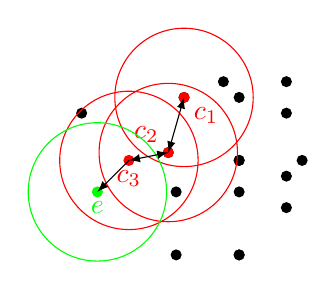
\begin{tikzpicture}
			\fill (-2,1.8) circle(2pt);
			\fill (-.9, 1.3) circle(2pt);
			\fill (-.8,.8) circle(2pt);
			\fill (-.8,0) circle(2pt);
			\fill (-.7,2) circle(2pt);
			\fill (-.2,2.2) circle(2pt);
			\fill (0,0) circle(2pt);
			\fill (0,1.2) circle(2pt);
			\fill (0,1.2) circle(2pt);
			\fill (0,0) circle(2pt);
			\fill (0,.8) circle(2pt);
			\fill (0,2) circle(2pt);
			\fill (.6,1) circle(2pt);
			\fill (.6,.6) circle(2pt);
			\fill (.6,1.8) circle(2pt);
			\fill (.6,2.2) circle(2pt);
			\fill (.8,1.2) circle(2pt);
			
			\fill[red] (-.7, 2) circle(2pt) node[anchor=north west]{$ c_1 $};
			\draw[red] (-.7, 2) circle(25pt);
			
			\fill[red] (-.9, 1.3) circle(2pt) node[anchor=south east]{$ c_2 $};
			\draw[red] (-.9, 1.3) circle(25pt);
			
			\fill[red] (-1.4,1.2) circle(2pt) node[anchor=north]{$ c_3 $};
			\draw[red] (-1.4,1.2) circle(25pt);
			
			\fill[green] (-1.8,.8) circle(2pt) node[anchor=north]{$ e $};
			\draw[green] (-1.8,.8) circle(25pt);
			
			\draw[latex-latex] (-.7, 2) -- (-.9, 1.3);
			\draw[latex-latex] (-.9, 1.3) -- (-1.4,1.2);
			\draw[-latex] (-1.4,1.2) -- (-1.8,.8);
		\end{tikzpicture}
		\subcaption{$ reach_{\varepsilon,\mu}(e, c_1) $} \label{fig:density-reachablity-reachability}
	\end{minipage}
	\begin{minipage}[b]{.5\linewidth}
		\centering
		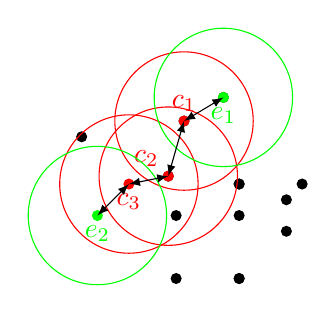
\begin{tikzpicture}
			\fill (-2,1.8) circle(2pt);
			\fill (-.9, 1.3) circle(2pt);
			\fill (-.8,.8) circle(2pt);
			\fill (-.8,0) circle(2pt);
			\fill (-.7,2) circle(2pt);
			\fill (-.2,2.3) circle(2pt);
			\fill (0,0) circle(2pt);
			\fill (0,1.2) circle(2pt);
			\fill (0,1.2) circle(2pt);
			\fill (0,0) circle(2pt);
			\fill (0,.8) circle(2pt);
			\fill (.6,1) circle(2pt);
			\fill (.6,.6) circle(2pt);
			\fill (.8,1.2) circle(2pt);
			
			\fill[red] (-.7, 2) circle(2pt) node[anchor=south]{$ c_1 $};
			\draw[red] (-.7, 2) circle(25pt);
			
			\fill[red] (-.9, 1.3) circle(2pt) node[anchor=south east]{$ c_2 $};
			\draw[red] (-.9, 1.3) circle(25pt);
			
			\fill[red] (-1.4,1.2) circle(2pt) node[anchor=north]{$ c_3 $};
			\draw[red] (-1.4,1.2) circle(25pt);
			
			\fill[green] (-1.8,.8) circle(2pt) node[anchor=north]{$ e_2 $};
			\draw[green] (-1.8,.8) circle(25pt);
			
			\fill[green] (-.2,2.3) circle(2pt) node[anchor=north]{$ e_1 $};
			\draw[green] (-.2,2.3) circle(25pt);
			
			\draw[latex-latex] (-.2,2.3) -- (-.7, 2);
			\draw[latex-latex] (-.7, 2) -- (-.9, 1.3);
			\draw[latex-latex] (-.9, 1.3) -- (-1.4,1.2);
			\draw[latex-latex] (-1.4,1.2) -- (-1.8,.8);
		\end{tikzpicture}
		\subcaption{$ connected_{\varepsilon,\mu}(e_1, e_2) $} \label{fig:density-reachablity-connection}
	\end{minipage}
	\caption{Relacje gęstościowej osiągalności \subref{fig:density-reachablity-reachability} oraz łączności \mbox{gęstościowej \subref{fig:density-reachablity-connection},} $ \mu = 3 $.}
\end{figure}

\definition{szum (ang. noise)}\newline
Punkt $ p $, który nie należy do żadnej z grup $ C_i $, nazywa się szumem\linebreak ($ noise_{D,\varepsilon,\mu}(p) $). Taki punkt $ p $ nie jest gęstościowo łączny z żadnym innym punktem $ q $.
\begin{equation}
	noise_{D,\varepsilon,\mu}(p) \iff \forall_i \;p\notin C_i \iff \forall_{q \in D} \,\neg connect_{D,\varepsilon,\mu}(p,q)
\end{equation}
	
\subsection{Algorytm}
Na podstawie przedstawionej wcześniej definicji grupy autorzy DBSCAN zaproponowali algorytm grupowania. Wersję tego algorytmu z drobną poprawką prezentuje \myhyperref{alg:dbscan}{algorytm}. Dla zachowania konsekwencji z linią 11 procedury $ expandcluster $ w linii 3 został dodany warunek $ cid(w) = unde\f{}ined $. W ten sposób zachowana jest poprawność wyniku, a $ \varepsilon $-otoczenie jest wyznaczane dla każdego punktu tylko raz, w odróżnieniu od oryginalnej propozycji, gdzie $ \varepsilon $-otoczenie może być wyznaczone więcej niż jeden raz dla tego samego punktu. Dalej nazwa DBSCAN będzie używana w odniesieniu do \myhyperref{alg:dbscan}{algorytmu}.

Okazuje się, że zgodnie z definicją grupy (\myhyperref{eq:cluster-def}{wyrażenie}) punkt $ p $ zbioru danych $ D $ może należeć do więcej niż jednej grupy. Taka sytuacja może mieć miejsce, gdy punkt $ p $ jest gęstościowo połączony z punktami $ q $ i $ r $, ale punkty $ q $ i $ r $ nie są ze sobą gęstościowo połączone.
\begin{equation}
  \left. \begin{array}{r}
		connected_{D,\varepsilon,\mu}(p, q) \\
		connected_{D,\varepsilon,\mu}(p, r) \\
		\neg connected_{D,\varepsilon,\mu}(q, r) \\
	 	q \in C_i \land r \in C_j
	\end{array} \right\}
	\implies	p \in C_i \cap C_j
\end{equation}
Stąd wynika, że punkt $ p $ musi być punktem brzegowym, ponieważ gdyby był punktem rdzeniowym, to $ q $ i $ r $ byłyby gęstościowo połączone za pośrednictwem $ p $.

Algorytm DBSCAN przypisuje każdy punkt ze zbioru danych do odpowiedniej grupy lub szumu poprzez nadanie punktom właściwych etykiet. Każdemu punktowi jest przypisywana tylko jedna etykieta, więc punkt może należeć do co najwyżej jednej grupy, stąd tworzone grupy nie są ściśle zgodne z definicją grupy (\myhyperref{eq:cluster-def}{wyrażenie}). Punkty brzegowe, które zgodnie z definicją grupy powinny należeć do więcej niż jednej grupy, są przez algorytm DBSCAN przypisywane tylko do jednej z tych grup. Co więcej, to, do której z grup zostanie przypisany punkt brzegowy, zależy od kolejności przetwarzania punktów zbioru danych.

Warto zwrócić uwagę, że $ \varepsilon $-otoczenie może być wyznaczane za pomocą dowolnej miary odległości lub podobieństwa\footnote{w przypadku miary podobieństwa należy w \myhyperref{eps-neighbourhood}{wyrażeniu} zanegować wartość miary lub odwrócić znak nierówności}. Najczęściej stosowane miary to odległość euklidesowa, Manhattan oraz podobieństwo kosinusowe.

\begin{algorithm}
 	\caption{DBSCAN \cite{dbscan}}\label{alg:dbscan}

	\DontPrintSemicolon
	
	\SetKwFunction{dbscan}{dbscan}
	\SetKwFunction{expand}{expandcluster}
	
	\setcounter{AlgoLine}{0}
	\nonl\SetKwProg{myproc}{Wejście}{}{}
	\myproc{}{
		$D$ - zbiór danych \;
		$\varepsilon $ - promień otoczenia \;
		$\mu $ - próg liczności otoczenia \;
	}
	\setcounter{AlgoLine}{0}
	\nonl\SetKwProg{myproc}{Wyjście}{}{}
	\myproc{}{
		każdy punkt zbioru $ D $ ma przypisaną etykietę grupy lub szumu\;
	}
	
	
	\setcounter{AlgoLine}{0}
	\nonl\SetKwProg{myproc}{Definicje}{}{}
	\myproc{}{
		$ nextcid() $ - zwraca nową unikalną etykietę grupy\;
		$ noise $ - etykieta szumu\;
		$ unde\f{}ined $ - nieokreślona etykieta\;
		$ cid(v) $ - etykieta punktu $ v $\;
		$ N_{V,\varepsilon}(v) $ - $ \varepsilon $-otoczenie punktu $ v $ w zbiorze $ V $ (\myhyperref{eps-neighbourhood}{wyrażenie})\;
		$ any(V) $ - dowolny element zbioru $ V $\;
		$ core_{V,\varepsilon,\mu}(v) $ - $ v $ jest punktem rdzeniowym w $ V $(\myhyperref{core-point}{wyrażenie})\;
	}
	\nonl\SetKwProg{myalg}{Algorytm}{}{}
	\myalg{\dbscan{$D$, $\varepsilon$, $\mu$}}{
		$ cid \gets nextcid() \;$ \tcp*{etykieta grupy}
		\ForEach{v \textbf{in} D}{
			\If{$ cid(v) = unde\f{}ined $}{
				\lIf{\expand{D, v, cid, $ \varepsilon $, $ \mu $}}{
					$ cid \gets nextcid() $
				}
			}
		}
	}
	\setcounter{AlgoLine}{0}
	\nonl\SetKwProg{myproc}{Procedura}{}{}
	\myproc{\expand{D, v, cid, $ \varepsilon $, $ \mu $}}{
		$ N_v \gets N_{D,\varepsilon}(v) $\;
		\uIf(\tcp*[f]{$ core_{D,\varepsilon,\mu}(v) $}){$ |N_v| \ge \mu $}{ 
			$ seeds \gets \set{w \in N_v | cid(w) = unde\f{}ined \land w \neq v} $\;
			\lForEach{$ w\ \mathbf{in}\ N_v $}{$ cid(w) \gets cid $}
			\While{$ seeds \neq \emptyset $} {
				$ w \gets any(seeds) $\;
				$ seeds \gets seeds \setminus \set{w} $\;
				$ N_w \gets N_{D,\varepsilon}(w) $\;
				\If($ \mathbf{foreach}\ x\ \mathbf{in}\ N_w $ \tcp*[f]{$ core_{D,\varepsilon,\mu}(w) $}){$ |N_w| \ge \mu $}{%
					\If{$ cid(x)\ \mathbf{in}\ \set{unde\f{}ined, noise} $}{
						\lIf{$ cid(x) = unde\f{}ined $}{$ seeds \gets seeds \cup \set{x} $}	
						$ cid(x) \gets cid $
					}
				}
			}
			\KwRet{true}\;
		}\Else{
			$ cid(v) \gets noise $\;
			\KwRet{false}\;
		}
	}
\end{algorithm}

\subsection{Wydajność}
Najbardziej czasochłonną operacją algorytmu DBSCAN jest wyznaczanie $ \varepsilon $-otoczenia punktu. Dla każdego punktu $ \varepsilon $-otoczenie wyznaczane jest co najwyżej raz\footnote{$ \varepsilon $-otoczenie punktu $ p $ jest wyznaczane tylko, jeśli etykieta punktu $ p $ jest nieokreślona, a  po wyznaczeniu $ \varepsilon $-otoczenia zawsze do $ p $ jest przypisywana etykieta}, dlatego jeśli za operację podstawową przyjmiemy wyznaczanie $ \varepsilon $-otoczenia, to w takim sensie złożoność algorytmu będzie liniowa.

Decydująca dla wydajnego działania DBSCAN jest optymalna implementacja wyznaczania $ \varepsilon $-otoczenia. Otoczenie można wyznaczać naiwnie, sprawdzając dla każdego punktu w zbiorze danych, czy znajduje się w $ \varepsilon $-otoczeniu punktu, dla którego jest poszukiwane $ \varepsilon $-otoczenie. Wyznaczanie $ \varepsilon $-otoczenia w ten sposób cechuje jednak liniowa złożoność względem liczby punktów w zbiorze danych, co przekłada się na złożoność kwadratową algorytmu DBSCAN. Istnieją metody pozwalające na wydajniejsze znajdowanie $ \varepsilon $-otoczenia i zostaną omówione w kolejnych rozdziałach.

Obliczanie wartości miary odległości lub podobieństwa jest czasochłonnym elementem wyznaczania otoczenia. Stosowane zazwyczaj miary wymagają liniowej liczby operacji względem wymiarowości zbioru danych. Wprowadza to liniową zależność czasu wyznaczania otoczenia od wymiarowości zbioru danych. Zakładając, że w podstawowym wariancie DBSCAN liczba operacji wyznaczania otoczenia jest kwadratowa względem rozmiaru zbioru danych, to za złożoność obliczeniową grupowania zbioru danych D można przyjąć $ \mathcal{O}(dim(D)|D|^2) $.